% ===== 分块 c02（源文件 QuantumWorkTry.tex 第 420--937 行）=====
% 内容：第 2 节 赝实费米子（§2 开头）、2.1 三维拓扑绝缘体（2.1.1--2.1.7）
% 说明：中文译注稿；公式、编号、引用与原文逐字对应；译者批注以 LaTeX 注释 [Tutor Note: ...] 的形式给出

\section{赝实费米子（Pseudoreal Fermions）}\label{pseudo}

\begin{keytakeaways}
\begin{itemize}[leftmargin=1.6em,itemsep=0.2em,topsep=0.2em]
  \item \textbf{物理图像}：三维拓扑绝缘体的边界是无质量的二分量狄拉克费米子；其路径积分的符号无法同时做到规范不变与时间反演不变，这种整体反常恰是体态电磁拓扑项取半周期值（即通常所说的“拓扑角等于圆周率”）的等价表述。
  \item \textbf{数学工具}：狄拉克算子的谱流、APS 指标定理及其指标公式、四维映射环面上的狄拉克指标、反射正定性，以及配边不变量（配边群到圆群的同态）。
  \item \textbf{核心结论}：体态相位与边界费米子相位相乘给出实数配分函数，其符号为负一的狄拉克指标次幂；该指标是配边不变量，因此自由费米子物相所对应的 sTQFT，其配分函数都是配边不变量。
\end{itemize}
\end{keytakeaways}

\subsection{三维拓扑绝缘体（Topological Insulator in $d=3$）}\label{topthree}

\subsubsection{基础（Basics）}

我们的第一个例子是 $d=3$ 中的拓扑绝缘体，本节在定向的 $3+1$ 维时空 $X$ 上研究它。
$X$ 带有空间边界，该边界是一个 $2+1$ 维可定向流形 $Y$。
拓扑绝缘体的边界模是一个 $2+1$ 维、无质量的二分量狄拉克费米子 $\psi$，其作用量为
\be\label{forx}I=\int_Y\d^3x \bar\psi \i\slashed{D}\psi.\ee
此处 $\slashed{D}=\sum_{\mu=0}^2\gamma^\mu D_\mu$ 是通常的狄拉克算子。$\psi$ 与电磁场的矢量势 $A$ 耦合，方式与电子相同；事实上，在能带理论中，$\psi$ 正是作为电子的一个模而出现的。
% [Tutor Note: 这里 $\i\slashed{D}$ 才是厄米算子：欧氏号差下 $\g^\mu$ 厄米而 $D_\mu$ 反厄米，故 $\i\slashed{D}$ 自伴、本征值实，这正是下文式（\ref{meto}）与“$\det\D$ 形式上是实数”的前提；若漏掉因子 $\i$，谱将整体为虚，符号问题无从谈起。]

还可以给 $\psi$ 赋予一个洛伦兹不变的质量项。此时狄拉克方程变为\footnote{在局部洛伦兹坐标中，我们的狄拉克矩阵是实矩阵，满足 $\{\g_a,\g_b\}=2\eta_{ab}$，其中 $\eta=\mathrm{diag}(-1,1,1)$。这些约定对于满足 $\sT^2=(-1)^F$ 的 $\sT$ 不变系统十分方便，并且使马约拉纳费米子与狄拉克费米子的比较变得直接。}
\be\label{orx}\left( \slashed{D}-m\right)\psi=0,\ee
其中 $m$ 为实数。这描述一个质量为 $|m|$、自旋为 $\frac{1}{2}\sign(m)$ 的粒子。时间反演与反射对称会反转粒子自旋的符号，因此对于 $m\not=0$，该微扰破坏 $\sT$ 与 $\sR$ 对称性。具体地说，一个 $\sT$ 变换\footnote{对马约拉纳费米子，我们必须考虑此方程中两种可能的符号：$\sT\psi(-t,x_1,x_2)=\pm\g_0\psi(-t,x_1,x_2)$。对具有 $\U(1)$ 对称性的狄拉克费米子，必要时可通过变换 $\psi\to\i\psi$ 消去这一符号。}
\be\label{rox}\sT\psi(t,x_1,x_2)=\g_0 \psi(-t,x_1,x_2) \ee
容易看出，它会使狄拉克方程中 $m$ 的符号反号。
% [Tutor Note: 原文“容易看出”这一步依赖 $\sT$ 反演中 $\g_0$ 的约定：按本页脚注，$\{\g_a,\g_b\}=2\eta_{ab}$ 且 $\eta=\mathrm{diag}(-1,1,1)$，故 $(\g_0)^2=-1$、$\g_0\g_i=-\g_i\g_0$。$t\to-t$ 把 $\partial_0$ 变为 $-\partial_0$，再把 $\g_0$ 移过 $\slashed{D}$ 时，$\g_0\g_0\g_0=-\g_0$ 与 $\g_0\g_i=-\g_i\g_0$ 恰好使动能项复原而质量项整体反号。注意此处的 $\g_0$ 是洛伦兹号差下的实矩阵（$(\g_0)^2=-1$），而下文转用欧氏号差后 $\gamma^\mu$ 全为厄米（$(\g^0)^2=1$），实现 $\sT$ 或反射的矩阵随之不同；两种约定下“$\sT$ 使 $m\to-m$”的结论相同，但若把两种约定的 $\g_0$ 混用，符号就会出错。]

然而，若我们有两个全同的狄拉克费米子 $\psi_1,\,\psi_2$，二者在 $\sT$ 下都按式（\ref{rox}）变换，则可以向狄拉克方程中加入一个 $\sT$ 不变的\footnote{式（\ref{worx}）中的质量项破坏 $\sR$，这里假定 $\sR$——一种空间反射——对 $\psi_1$ 与 $\psi_2$ 的作用方式相同，即 $\sR\psi_i(t,x_1,x_2)=\pm \g_1\psi_i(t,-x_1,x_2)$。（该质量项保持的是另一种 $\sR$ 对称性。）相对论性 QFT 中唯一的普适对称性是 $\sCRT$，这意味着 $\sT$ 对称性等价于 $\sCR$ 对称性。给定一个 $\sT$ 对称性，就有一个典范的 $\sCR$ 对称性，但并不存在典范的 $\sR$ 对称性。}质量项：
\be\label{worx}\left(\slashed{D}-\bp 0 & \i m \cr -\i m & 0\ep\right)\bp \psi_1\cr \psi_2\ep=0 . \ee
将质量项对角化可以看出，$\sT$ 交换两个质量（与电荷）相同、自旋相反的模。既然单个狄拉克费米子无法获得保持 $\sT$ 的质量，由此可知：在 $3+1$ 维中，若一个 $\sT$ 不变的材料在其边界上只有一个无质量狄拉克费米子，则这一状况受 $\sT$ 不变性保护。本段我们用洛伦兹号差书写，因为这使 $\sT$ 的作用最为透明；但在下文对 $\psi$ 的路径积分及其反常的分析中，我们取 $Y$ 为欧几里得号差。
% [Tutor Note: 式（\ref{worx}）的 $2\times2$ 质量矩阵本征值为 $\pm m$，本征矢为 $\psi_1\pm\i\psi_2$：$\sT$ 把 $+m$ 模映到 $-m$ 模，故单费米子无从获得保持 $\sT$ 的质量，而两个费米子可以。这正是 $3+1$ 维 $\sT$ 不变拓扑绝缘体边界只能有奇数个狄拉克锥的“配对”论证。]

$\psi$ 场的路径积分 $Z_\psi$ 形式上就是算子 $\D=\i\slashed{D}$ 的行列式：
\be\label{deto}Z_\psi=\det\,\D.\ee
算子 $\D$ 是厄米的，故其本征值为实数：
\be\label{meto}\D\psi_i=\lambda_i\psi_i,~~\lambda_i\in\R.\ee
形式上，行列式就是本征值的乘积：
\be\label{peto}\det\,\D=\prod_i\lambda_i.\ee

形式上这是实数，因为所有因子都是实数。
这一实数性有简单的物理含义：它反映了我们试图量子化的经典场论的 $\sT$ 不变性。
一般地，在任何幺正的 QFT 中，在欧几里得号差的定向时空 $X$ 上，若把 $X$ 的定向反转，则配分函数变为其复共轭。
在 $\sT$ 不变的理论中，这种定向反转是一种对称性，因此配分函数总是实数。这一切只对可定向的 $X$ 成立；对不可定向的 $X$，$\sT$ 不变性并不要求配分函数为实数。例子见第 \ref{complex} 节。
% [Tutor Note: 这里“形式上”三字不能略过：$\prod_i\lambda_i$ 是无穷乘积，既无自然正规化，也不绝对收敛；本节的整条论证线索——谱流、$\eta$ 不变量、$(-1)^\iota$——正是为了给这个无穷乘积的符号赋予严格定义。]

对于{\it 两个}无质量狄拉克费米子，路径积分将是
\be\label{reto}Z_\psi^2=\prod_i\lambda_i^2. \ee
每个因子不仅是实数而且是正数，故形式上人们当然预期 $Z_\psi^2$ 为正；事实上，两个无质量狄拉克费米子的路径积分可以自然地定义为正。
既然为正，它就等于 $|Z_\psi|^2$，从而是完全无反常的——因为正如我们在第 \ref{generalities} 节所解释的，相对论性费米子路径积分的绝对值 $|Z_\psi|$ 总可以以一种完全无反常、保持一切对称性的方式定义。
特别地，$Y$ 上两个无质量狄拉克费米子的路径积分可以按 $\sT$ 不变的方式定义。
这并不奇怪，因为上文已经看到，$\sT$ 不变的质量项、从而 $\sT$ 不变的泡利--维拉尔斯正规化子是存在的。（$\sT$ 不变的泡利--维拉尔斯正规化基于 $\sT$ 不变的有质量狄拉克方程（\ref{worx}），因此它对两个狄拉克费米子的一个线性组合使用正质量正规化子，对另一个使用负质量正规化子。）

然而，只有一个狄拉克费米子时就有麻烦了，因为形式表达式
\be\label{wink}Z_\psi=\prod_i\lambda_i \ee
天然是实数，却并非天然为正。它的符号粗略地说等于负的 $\lambda_i$ 的个数模 2，但负的 $\lambda_i$ 有无穷多个，而没有任何自然的方式判定这个无穷数是偶数还是奇数。
% [Tutor Note: “负本征值个数模 2”只是启发性说法：$\lambda_i\to-\lambda_i$ 的配对（由某个反交换的反射/手征算子给出）使相邻谱的贡献成对抵消，剩下的正是模 2 指标。对单个狄拉克费米子，这个模 2 信息不能由任何局部泛函给出，只能由四维狄拉克指标 $\iota$ 给出——见式（\ref{torf}）。]
% [Tutor Note: 本节处理的是带 $\U(1)$ 对称性的狄拉克费米子，路径积分是行列式 $\det\D$，其符号等于负本征值个数的奇偶性。对马约拉纳费米子（见 2.2.1 小节“Fermions And Pfaffians”）则没有守恒的 $\U(1)$，路径积分只能写成 Pfaffian；此时谱成 $\pm\lambda$ 配对，Pfaffian 在每一对穿过零点时变号，符号歧义比行列式情形更突出，但处理手法（谱流加四维指标）完全相同。]

\subsubsection{整体反常与谱流（Global Anomaly And Spectral Flow）}\label{trada}

事实上，如果我们试图把 $Z_\psi$ 定义为正的且规范不变的，就会陷入矛盾。
我们可以任取一个度规与规范场，比如 $g=g_0$ 与 $A=A_0$，并规定 $Z_\psi$ 在 $(A,g)=(A_0,g_0)$ 处为正。
然后让 $A$ 与 $g$ 变化，我们便可连续地追踪 $Z_\psi$ 的符号，并规定：每当 $\D$ 的一个本征值穿过 0 时，该符号就改变。
然而，这一做法与规范不变性相冲突。
设 $\phi$ 为一个规范变换，或一个规范变换与一个微分同胚的组合。
设 $(A_0^\phi,g_0^\phi)$ 为 $A_0$ 与 $g_0$ 在 $\phi$ 下所变成的对象。
我们总能从 $(A_0,g_0)$ 连续插值到 $(A_0^\phi,g_0^\phi)$：引入实参数 $s$，$0\leq s\leq 1$，然后令
\be\label{zink}A_s=(1-s)A_0+sA_0^\phi,~~~ g_s=(1-s)g_0+sg_0^\phi. \ee
这些式子取得使 $(A_s,g_s)$ 在 $s=0$ 处与 $(A_0,\phi_0)$ 重合、在 $s=1$ 处与 $(A_0^\phi,g_0^\phi)$ 重合。
在接受这个从 $(A_0,\phi_0)$ 到 $(A_0^\phi,g_0^\phi)$ 的插值之前，我们应当确认 $A_s$ 与 $g_s$ 对一切 $s$ 都有良好定义。
度规 $g_s$ 理应正定。这没有问题，因为当 $0< s< 1$ 时，$g_s$ 是正度规 $g_0$ 与 $g_0^\phi$ 的、系数为正的线性组合。
至于 $A_s$，其实并没有类似的条件需要检验。
% [Tutor Note: 原文此处（源行 87--88 附近）两次写作 $(A_0,\phi_0)$，按上下文应为 $(A_0,g_0)$：插值式（\ref{zink}）在 $s=0$ 处应回到起点 $(A_0,g_0)$，而 $\phi$ 是规范变换/微分同胚，$\phi_0$ 并不是这里的场变量。译文保留原式，以便与原文逐字对照。]

\begin{figure}[htbp]
  \centering
  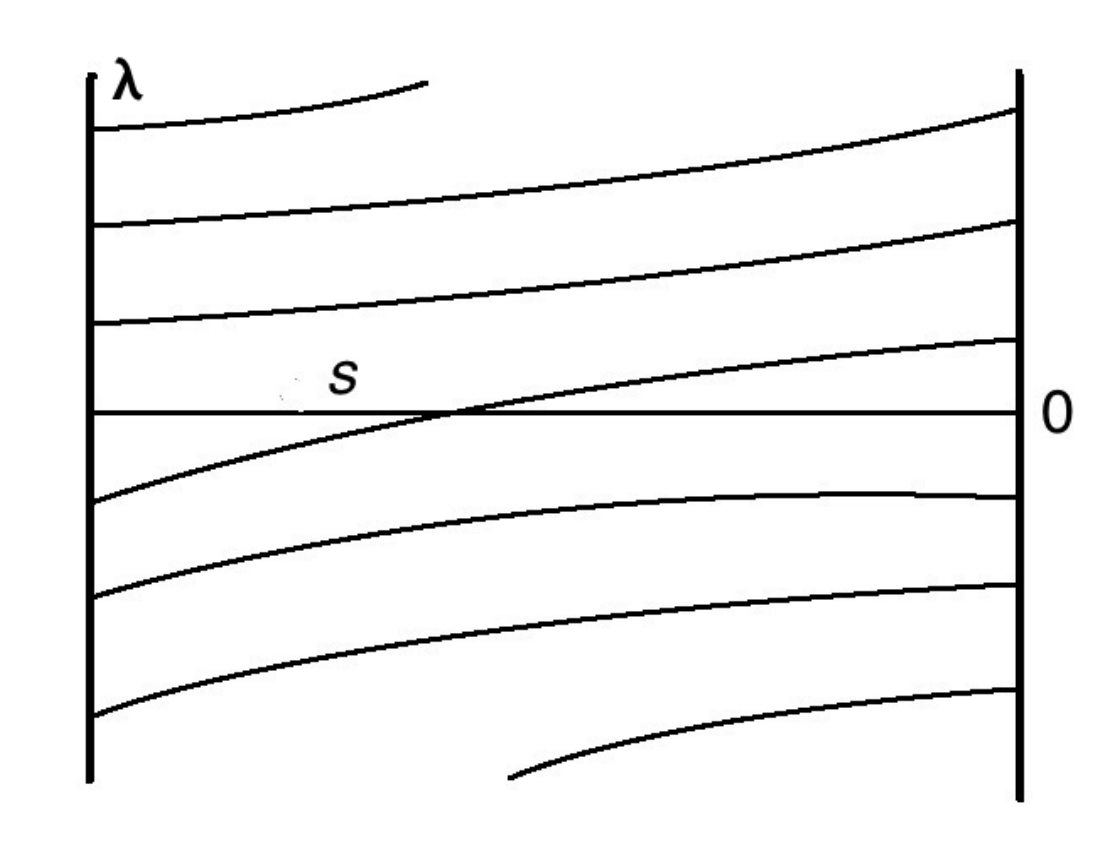
\includegraphics[width=0.55\textwidth]{fig01.png}
  \caption{狄拉克算子的谱流。竖直轴表示本征值 $\lambda$，水平轴表示本征值所依赖的参数 $s$。图中所示情形下，谱在 $s=1$ 处与在 $s=0$ 处相同，但在 $s=0$ 与 $s=1$ 之间有一个本征值净向上穿过 $\lambda=0$。这导致费米子路径积分 $Z_\psi$ 变号。（原文第 14 页，图 1）}
  \label{flow}
\end{figure}

现在让 $(A_s,g_s)$ 从 $s=0$ 连续演化到 $s=1$，并考察 $Z_\psi$ 变号多少次。
规范不变性要求 $Z_\psi$ 在 $s=1$ 处的符号应与 $s=0$ 处相同，因为 $s=1$ 处的 $(A_s,g_s)$ 与 $s=0$ 处规范等价。
然而，一般而言这里有问题：规范不变性只要求狄拉克算子在 $s=1$ 处的谱与 $s=0$ 处相同，但在 $s=0$ 与 $s=1$ 之间，狄拉克本征值可以出现净的“谱流”，如图 \ref{flow} 所示。
这种谱流之所以可能，正是因为 $\D$ 具有无穷多个正本征值与负本征值。
% [Tutor Note: 图 \ref{flow} 的对角线只画出一个本征值向上穿过零点，但物理上要点是“净”流量：任意一对正负本征值可以成对穿过零点而不留下拓扑痕迹，只有净流量 $\Delta$ 才进入配分函数的符号。这正是后文把符号问题归结为四维指标 $\iota$ 的原因。]

就三维拓扑绝缘体的边界费米子而言，若期望 $Z_\psi$ 为实数，则在定义其符号时确实存在这种不相容性。
穿过 $\lambda=0$ 的本征值净数目 $\Delta$ 其实有一个拓扑公式，即
\be\label{worf}\Delta=\iota,\ee
其中 $\iota$ 是某个 $D=4$ 中的狄拉克指标，稍后即会说明。
相应地，$Z_\psi$ 在 $s=0$ 与 $s=1$ 之间的变号公式为
\be\label{torf}Z_\psi\to Z_\psi (-1)^\iota.\ee
$\iota$ 将是某个四维流形 $X$ 上的狄拉克指标，此流形称为映射环面。
该流形是研究 $Y$ 上费米子理论中反常的一个计算工具。
在关于拓扑绝缘体的讨论中，四维流形一般就记作 $X$，无论它是研究反常的工具，还是物理系统的世界体。
理由是：两种情形会用到相同的数学考量。
这并非巧合，而体现了边界反常在拓扑绝缘体物理中的重要性。
% [Tutor Note: 式（\ref{worf}）中的 $\Delta$ 是“净”谱流，即向上穿过零点的本征值数减去向下穿过者；由于谱在 $s=1$ 与 $s=0$ 相同，这个净数只能是整数 $\iota$。原文“as described momentarily”指的是下一步用映射环面 $X$ 上的 4 维狄拉克指标来定义它。]

为定义 $X$，令 $I$ 为单位区间 $0\leq s\leq 1$。
我们用微分同胚 $\phi$ 把 $I\times Y$ 的两端黏合起来，构造一个无边的四维流形 $X$。\footnote{可以略微修改度规对 $s$ 的依赖，使 $X$ 上的度规在端点 $s=0$ 与 1 处光滑。}
以这种方式构造的流形称为映射环面。
再利用 $\phi$ 中规范变换的部分，把 $I\times Y$ 两端处的规范丛黏合起来，得到 $U(1)$ 规范丛 $\L\to X$。
于是 $\iota$ 就是 $X$ 上、与 $\L$ 耦合的 4 维狄拉克算子的指标\footnote{\label{helpful}我们不必在紧致的映射环面 $X$ 上工作：可以令 $u=1/(1-s)-1/s=(2s-1)/s(1-s)$，于是 $0<s<1$ 对应于 $-\infty<u<\infty$，并在非紧的四维流形 $X'\cong\R\times Y$ 上工作，其度规为 $\d u^2+ g_{s(u)}$，相应的规范场则依赖 $u$，记为 $A_{u(s)}$。在平方可积波函数空间中，$X'$ 上狄拉克算子的指标与 $X$ 上的指标相同。}。
（狄拉克指标的定义见第 \ref{why} 节。）
三维谱流与四维狄拉克指标之间的这一关系最初在 \cite{APS} 中得到，它在 QCD 中有应用，物理学文献中也已有描述 \cite{DCG,Kiskis}。

上面所描述的、即把 $Z_\psi$ 的符号或相位视为参数 $s$ 的函数并寻找可能的不相容性，正是 20 世纪 80 年代 \cite{Witold,Witoldtwo,Global} 研究整体反常的框架。
人们一度以为这就是故事的全部。如今已经清楚并非如此，本文需要一个更完整的处理。
我们从传统框架开始，并不是要去追溯历史，而是因为这是引入重要拓扑不变量最初步的方式——尤其是本例中的指标 $\iota$，以及后文例子中它的类似物。

传统框架所缺少的东西可以这样描述。$Z_\psi$ 的符号没有反常，意味着在某个给定的 $Y$ 上，$Z_\psi$ 作为 $(A,g)$ 的函数有良好定义，至多相差一个只依赖于 $Y$、而不依赖于 $(A,g)$ 的整体符号。
（在上述论证中，这个符号被取作 $Z_\psi$ 在某个任意起点 $(A_0,g_0)$ 处的符号。）
但我们需要一种确定这个整体符号的办法；若对每个 $Y$ 独立地定义 $Z_\psi$ 的符号，那就肯定不能指望得到一个令人满意的理论。
一个确定的物理理论对这些符号给出确定的答案。
物理上，在各种切割与黏合操作下——即把各个三维流形 $Y_i$ 切成碎片、再以不同方式黏合起来——理论必须有合理的行为。
% [Tutor Note: 这一段是理解“整体反常”的关键：传统框架只能保证 $Z_\psi(A,g)$ 在固定 $Y$ 上相差一个与 $(A,g)$ 无关的常数符号；真正要定义的是这个常数，而它必须与流形的切割黏合相容。这个要求比单点规范不变性更强，也是下一段量子力学类比要说明的。]

这类切割关系的原型出现在普通量子力学中：设哈密顿量为 $H$；若把长度为 $t$ 的时间区间分解为长度 $t_1$ 与 $t_2$ 的两个相继区间，其中 $t=t_1+t_2$，则有 $\exp(-\i Ht)=\exp(-\i Ht_2)\exp(-\i Ht_1)$，由此得到关于跃迁振幅的一个著名结果
\be\label{cutting}\langle f|\exp(-\i Ht)|i\rangle
=\sum_k \langle f|\exp(-\i H t_2)|k\rangle \langle k|\exp(-\i Ht_1)|i\rangle,\ee
其中对中间态求和。这在任意维度的量子场论中都有类比：把一个流形切成若干块，并断言整个流形上的路径积分等于各块上路径积分的乘积（在黏合处对物理态求和）。
量子场论的情形比量子力学丰富得多，因为在更高维中把流形切成碎片的办法要多得多。
与切割和黏合的相容性，正是量子场论局域性的本质。

在与拓扑物态相关的情形中——三维拓扑超导体就是一个好例子——即使不存在传统意义上的反常（即在一个特定 $Y$ 上定义路径积分并无不相容），也可能存在更微妙的整体反常：无法在不同 $Y$ 上令人满意地定义路径积分的整体符号或相位。
必须把这些更微妙的整体反常纳入范式“$d$ 维的反常 $\longleftrightarrow$ $d+1$ 维的 SPT 相”之中。
把这些整体反常考虑在内，意味着要为每个 $Y$ 与每组 $(A,g)$ 绝对地定义费米子路径积分 $Z_\psi$ 的符号。
接下来我们将照此办理，做法遵循 \cite{ADM}。

\subsubsection{$\sT$ 反常（T Anomaly）}\label{zelfan}

对 $2+1$ 维狄拉克费米子 $\psi$ 而言，定义 $Z_\psi$ 的符号时存在困难，这并不意味着该理论自相矛盾。
它只意味着，该理论无法按 $\sT$ 不变（或 $\sR$ 不变）的方式量子化。
只要我们不去追求 $Z_\psi$ 为实数，就可以一致地定义它。

毕竟，$\psi$ 可以带有规范不变的裸质量，这会破坏 $\sT$ 对称性，除此之外在物理上完全可以接受。
存在破坏 $\sT$ 的质量，意味着我们可以牺牲 $\sT$ 对称性，通过引入泡利--维拉尔斯正规化子场 $\chi$ 来正规化该理论；可以把它看作一个玻色场，它满足有质量狄拉克方程 $(\i\slashed{D}+\i\mu)\chi=0$，其中 $\mu$ 非常大。
在欧几里得号差下，正规化后的路径积分为
\be\label{pv} Z_{\psi,\,\reg}=\prod_k\frac{\lambda_k}{\lambda_k+\i \mu}. \ee
其实，我们写下的式子虽然足以满足当前目的，却只是泡利--维拉尔斯手续的一种近似。
一般而言，人们会引入多种有质量玻色场与费米场，其质量 $\mu_a, \,a=1,\dots, t$ 各不相同且都很大，并选取它们使正规化后的路径积分对固定的 $\mu_a$ 收敛。
然后取极限 $\mu_a\to\infty$，同时向作用量中加入局部抵消项 $W(\mu_a, A,g)$，使 $Z_{\psi,\,\reg}\exp(-W(\mu_a,A,g))$ 的极限存在。
该极限就是重整化后的费米子路径积分。
我们无需详细遵循这一手续，因为我们只关心 $Z_\psi$ 的相位，而式（\ref{pv}）已足以启发该相位的正确公式。（3 维时空所需的抵消项全为实数，不影响关于相位的讨论。）
% [Tutor Note: 式（\ref{pv}）中被积掉的正是正规化子的“质量符号”：$\lambda_k/(\lambda_k+\i\mu)$ 在 $\mu\to\infty$ 时给出 $\mp\i$ 的相位，其符号只依赖 $\lambda_k$ 的正负。这里用复质量 $\i\mu$ 是为了让乘积在欧氏号差下收敛；换成 $-\i\mu$ 就得到式（\ref{yv}）的共轭相位，这正是 $\sT$ 破缺的来源。]

回到式（\ref{pv}），可见当 $\mu>0$ 很大时，每个本征值 $\lambda_k$ 都向 $Z_\psi$ 贡献一个相位 $\i^{-1}$ 或 $\i$，视 $\lambda_k$ 的符号而定。
于是形式上
\be\label{nv}Z_\psi=|Z_\psi|\exp\left(-\frac{\i\pi}{2}\sum_k \sign(\lambda_k)\right). \ee
因此
\be\label{mv} Z_\psi=|Z_\psi|\exp\left(-\i\pi\etta/2\right), \ee
其中 $\etta$（即 Atiyah--Patodi--Singer 或 APS $\etta$ 不变量）是 $\D$ 的正、负本征值数目之差的某种正规化版本\footnote{\label{later} 在目前的推导中，$\lambda_k$ 是作用在带正电的狄拉克费米子 $\psi$ 上的狄拉克算子 $\D$ 的本征值，并未计入作用在带负电的场 $\bar\psi$ 上的 $\D$ 的电荷共轭本征模。我们也可以定义类似的不变量 $\eta$，其中对两种模都求和。由电荷共轭对称性，两者之间的关系就是 $\eta=2\etta$。后文讨论马约拉纳费米子时（没有 $\U(1)$ 对称性，因而正负电荷的模没有区别），我们会希望把所有公式都用 $\eta$ 表示。}。
% [Tutor Note: 式（\ref{mv}）中的因子 $1/2$ 极易出错：$\etta$ 是“正负本征值数之差”的正规化值，每穿过一次零点跳变 $\pm2$，故相位为 $\exp(-\i\pi\etta/2)$ 时才会在零点处精确变号（$e^{\mp\i\pi}=\pm1$ 的符号）。若把定义写成不含 $1/2$ 的形式，后文式（\ref{sv}）与 APS 公式（\ref{wont}）的指数都会差一倍。]

与通常一样，具体的正规化方式无关紧要。APS 原来的定义是\footnote{这个定义需要某种解析延拓：先对大的 $\mathrm{Re}\,s$ 定义式（\ref{rv}）右端的求和，此时它收敛；然后解析延拓到 $s=0$。注意式（\ref{rov}）中的替代定义不需要这种解析延拓。}
\be\label{rv}\etta=\lim_{s\to 0}\sum_k\sign(\lambda_k)|\lambda_k|^{-s}. \ee
一个等价的定义是
\be\label{rov}\etta=\lim_{\veps\to 0^+}\sum_k\sign(\lambda_k)\exp(-\veps\lambda_k^2). \ee
就目前的应用而言，我们不需要知道当 $\lambda=0$ 时 $\sign(\lambda)$ 是什么意思，因为若某个 $\lambda_k$ 为 0，则 $|Z_\psi|=0$，此时给 $\etta$ 赋什么值都无所谓。
不过，如果在 $\etta$ 的定义中取
\be\label{uv}\sign(\lambda)=\begin{cases} 1 &  \text{if}~\lambda\geq 0\cr -1&\text{if}~\lambda<0. \end{cases}.\ee
则指标理论的公式会运作得很顺畅。取 $\lambda=0$ 时 $\sign(\lambda)=-1$ 也同样可行；要点在于以相同方式处理所有零模。

公式
\be\label{sv}Z_\psi=|Z_\psi|\exp(-\i\pi\etta/2), \ee
连同任何定义 $|Z_\psi|$ 的标准手续，给出了 $Z_\psi$ 对一切 $Y$、一切 $A,g$ 的满意定义，具备除 $\sT$ 与 $\sR$ 对称性之外的所有合意性质。
$\sT$ 与 $\sR$ 对称性并不成立，因为它们要求 $Z_\psi$ 为实数。
$\sT$ 与 $\sR$ 对称性已被正规化子质量的符号选择所破坏。
若取相反符号，同样好的正规化会给出 $Z_\psi$ 的相反相位，因此我们实际上有两个同样好的定义：
\be\label{yv}Z_\psi=|Z_\psi|\exp(\mp \i\pi\etta/2). \ee
这两个公式中的任何一个，都在背景场 $(A,g)$ 中给出一个无能隙自由费米子 QFT 的配分函数；该 QFT 完全幺正、庞加莱不变——甚至共形不变——并且在其他方面物理上合理，但并不具有 $\sT$ 或 $\sR$ 不变性。

为结束本节，我们将解释“路径积分的公式（\ref{yv}）在物理上是合理的”这一陈述的若干方面。
费米子路径积分 $Z_\psi$ 应当在费米子本征值穿过 0 时变号。公式（\ref{sv}）确实具有这一性质。
第一个因子 $|Z_\psi|$ 当然不变号，而第二个因子 $\exp(\mp \i\pi\etta/2)$ 确实变号，因为当本征值穿过 0 时 $\etta$ 跳变 $\pm 2$。

我们也许还想验证配分函数的定义与幺正性相容。
在欧几里得号差下，幺正性对应反射正定性。
设 $Y_1$ 与 $Y_2$ 是两个全同的三维流形，赋有相同的规范场与自旋结构，并设 $M$ 是它们的公共边界。
把 $Y_1$ 与 $Y_2$ 沿 $M$ 黏合起来（先反转 $Y_2$ 的定向以使两者定向匹配），构造一个三维流形 $Y$。
这一构造示于图 \ref{dodo}。在此情形下 $Z_\psi$ 应当是实数且非负的，理由如下：$Y_1$ 上的路径积分在 $M$ 上量子态的希尔伯特空间中构造出一个态 $|\Phi\rangle$，即一个“右矢”；$Y_2$ 上的路径积分在同一希尔伯特空间中构造出相应的“左矢” $\langle\Phi|$。$Y$ 上的完整路径积分 $Z_\psi$ 就是内积 $\langle\Phi|\Phi\rangle$。在幺正的量子场论中，这当然是实数且非负的。
% [Tutor Note: 这一段把反射正定性与“把流形沿边界黏合”等同起来：物理上 $Z_\psi=\langle\Phi|\Phi\rangle\ge 0$ 正是希尔伯特空间内积的正定性。原文随后用 $\etta$ 的谱对称性来证明这一点，等价于说：反射对称使谱成 $\pm\lambda$ 配对，从而 $\etta=0$、相位因子为 1。]

要证明 $Z_\psi\geq 0$，只需证明在此情形下 $\exp(\mp \i\pi \etta/2)$ 等于 1，只要没有零模（即只要 $|Z_\psi|\not=0$）。
这是对的，因为交换 $Y_1$ 与 $Y_2$ 并反转 $Y$ 定向的那个反射，与狄拉克算子反交换，而该算子为 $\D=\i\slashed{D}=\i\sum_{\mu=1}^3\g^\mu D_\mu.$
例如，若 $Y=\R^3$ 取平直度规，则反射
\be\label{refact}\sR\psi (x_1,x_2,x_3)=\g^1\psi(-x_1,x_2,x_3) \ee
显然与 $\slashed{D}$ 反交换。事实上，对奇数维流形上任何反转定向的对称性，这都是普遍结论。
因此图 \ref{dodo} 中的反射对称性意味着狄拉克算子的本征值在 $\lambda\leftrightarrow -\lambda$ 下不变，而这又意味着（在没有零模时）$\etta=0$ 且 $\exp(\mp \i\pi\etta/2)=1$。
% [Tutor Note: 反射与 $\D$ 反交换的证明只需一维：$\sR$ 反转 $x_1$，使 $\partial_1\to-\partial_1$；而 $\sR$ 用 $\g^1$ 实现，$\g^1\g^1\g^1=\g^1$、$\g^1\g^i=-\g^i\g^1$（$i\ne1$），故 $\sR\D\sR^{-1}=-\D$。于是 $\D$ 与 $-\D$ 谱相同，正负本征值一一配对、$\etta=0$。注意这里 $\g^1$ 是厄米矩阵，与前面马约拉纳情形所用的反厄米 $\g_0$ 不同。]

反转时空定向的对称性与狄拉克算子反交换，正是加入狄拉克方程的质量项会破坏这类对称性的原因。
显然，如果 $\sR$ 与 $\i\slashed{D}$ 对易，那么有质量狄拉克方程——在欧几里得号差下应为 $\left(\i\slashed{D}+\i m\right)\psi=0$——就会是 $\sR$ 不变的。

\begin{figure}[htbp]
  \centering
  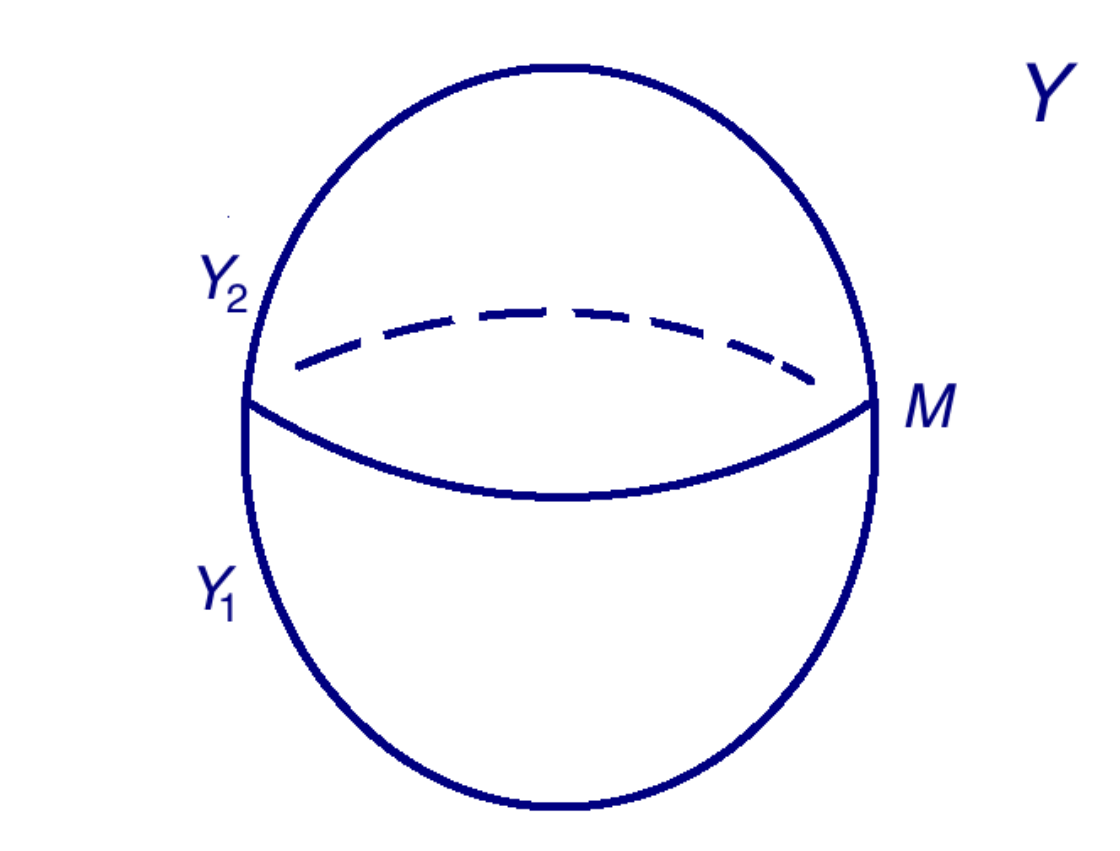
\includegraphics[width=0.55\textwidth]{fig02.png}
  \caption{三维流形 $Y$ 的镜像对称构造：把全同的两块 $Y_1$ 与 $Y_2$ 沿其公共边界 $M$ 黏合起来，其中 $Y_2$ 的定向取反。（原文第 19 页，图 2）}
  \label{dodo}
\end{figure}

\subsubsection{抵消来自体态的反常（Canceling The Anomaly From The Bulk）}\label{canbulk}

刚才讨论的、三维拓扑绝缘体边界费米子破坏 $\sT$ 不变性的反常，与下述事实 \cite{ZQH} 有关：在体态中，这种材料具有等于 $\pi$ 的电磁 $\theta$ 角。

四维时空中 $\U(1)$ 规范场的瞬子数定义为
\begin{equation}\label{zelm}P=\frac{e^2}{32\pi^2}\int_X \d^4x\,\epsilon^{\mu\nu\alpha\beta}F_{\mu\nu}F_{\alpha\beta},\ee
其中 $F_{\mu\nu}=\partial_\mu A_\nu -\partial_\nu A_\mu$ 是电磁场强。
若 $X$ 是带边的紧致流形，则 $P$ 总是整数。
$P\not=0$ 的典型例子是 $X=S^2\times S^2$，且其中每个因子各带一个单位磁通（即 $\int_{S^2}F=2\pi/e$）。该例子给出 $P=1$。
% [Tutor Note: 归一化约定值得注意：磁通量子取 $2\pi/e$（取 $\hbar=1$），于是 $e^2/(32\pi^2)\int \epsilon^{\mu\nu\alpha\beta}F_{\mu\nu}F_{\alpha\beta}$ 在 $S^2\times S^2$ 上每个因子带单位磁通时恰给出整数 $1$。若 $e$ 的约定改变，$P$ 会差一个整数因子，$\theta$ 的周期也随之改变。]

电磁 $\theta$ 角由下式定义：有效作用量中依赖于 $P$ 的部分为
\be \label{zpart}I_\theta=\theta P.\ee
若可以假定 $P$ 取整数值，则物理在 $\theta\to\theta+2\pi$ 下不变，因为在量子力学中我们只关心作用量的值模 $2\pi\Z$。
% [Tutor Note: 这里“$P$ 为整数”是 $\theta$ 周期为 $2\pi$ 的前提；一旦时空有边界或拓扑绝缘体只占据时空的一部分，$P$ 不再取整，$\theta$ 的周期性论证便失效——这正是下一段要处理的问题，也是“体内 $\theta=\pi$”必须配合边界态才有意义的原因。]

$P$ 在反射或时间反演下为奇，故 $\theta$ 同样为奇。
在 $\sT$ 或 $\sR$ 不变的理论中，$\theta$ 必须等于 0 或 $\pi$（$\sT$ 与 $\sR$ 把 $\theta=\pi$ 映为 $\theta=-\pi$，后者与 $\theta=\pi$ 模 $2\pi$ 等价）。
文献 \cite{ZQH} 证明：假定真空中 $\theta=0$，则三维拓扑绝缘体内部 $\theta=\pi$。
\ 

然而，真实的拓扑绝缘体有边界，其世界体 $X$ 并不填满整个时空。
此时 $P$（定义为对 $X$ 而非对整个时空的积分）一般不是整数。
因此，仅在路径积分中乘入一个因子 $\exp(\pm \i\pi P)$ 并不具有 $\sT$ 不变性。
在可定向时空上，$\sT$ 不变性要求路径积分的被积量应为实数，而当 $P$ 不取 $\Z$ 值时，$\exp(\pm \i\pi P)$ 显然不具备这一性质。
作用 $\sT$ 会使指数 $\exp(\pm\i\pi P)$ 中的符号反转。

更具体地说，若在有拓扑绝缘体存在时直接向泛函积分中乘入因子 $\exp(\pm \i \pi P)$，则由一个众所周知的论证，这会在拓扑绝缘体表面产生霍尔电导 $\nu=\pm 1/2$（照例，$\nu$ 是以 $e^2/2\pi\hbar$ 为单位的霍尔电导）。这当然不保持 $\sT$。
% [Tutor Note: 表面霍尔电导 $\nu=\pm 1/2$ 的来源是 $\theta$ 项在边界处的“反常流入”：$\theta$ 从内部的 $\pi$ 变到外部的 0，$\partial_\mu\theta$ 在边界上给出一个 Chern--Simons 型表面项，其系数正是半整数量子化。原文用“众所周知的论证”带过，细节可参看 \cite{ZQH}。]

在拓扑绝缘体的语境中，“$\theta=\pi$ 保持 $\sT$”这一断言实际意味着：它在体态中保持 $\sT$，并且只要我们找到正确的边界态，就有可能沿边界维持 $\sT$ 不变性。
平庸的有能隙边界态并不合适。

然而，带有无质量狄拉克费米子的标准边界态确实能与 $\theta=\pi$ 的体态结合，从而维持 $\sT$ 对称性。
我们回顾一下，边界费米子的配分函数为
\be\label{dont} Z_\psi=|Z_\psi|\exp(\mp\i\pi\etta/2),\ee
其中符号取决于正规化子的选择。
结果表明，若从 $P$ 中减去一个引力修正——暂且只记作 $\hA(R)$\footnote{我们用 $\hA(R)$ 作为更常见的 $\int_X\hA(R)$ 的缩写。}——则 $\theta=\pi$ 时路径积分的体态贡献与边界费米子的配分函数相结合，给出保持 $\sT$ 的结果。
事实上，根据 Atiyah、Patodi 与 Singer（APS）\cite{APS}，
\be\label{wont}\exp(\mp\i\pi\etta/2)\exp\left(\pm \i\pi(P-\hA(R))\right)=(-1)^\iota,\ee
其中 $\iota$ 为整数。
正如我们在第 \ref{aps} 节所解释的，$\iota$ 是按 APS 边界条件计算的狄拉克算子的指标。
因此，积分掉边界费米子之后，完整的路径积分测度为
\be\label{ont}|Z_\psi|\exp(\mp\i\pi\etta/2)\exp\left(\pm \i\pi(P-\hA(R))\right)=|Z_\psi|(-1)^\iota. \ee
（该公式本质上已在 \cite{MW} 第 5.3 节关于弦论中 D-膜的相关讨论中得到。）这是实数，故保持 $\sT$。
% [Tutor Note: 式（\ref{wont}）就是 APS 指标定理在带边四维流形上的形式：左端是 $\eta$ 不变量的相位与 $\theta$ 项（含 $\hA$ 引力修正）的相位之积，右端是整数指标的符号 $(-1)^\iota$。关键点是两个看似非整数的相位相乘后必为 $\pm1$：$\eta$ 的分数部分被 $P-\hA(R)$ 精确抵消。需要强调的是，$\hA(R)$ 必须相对于同一度规计算，否则抵消不成立。]

本节余下部分，我们讨论公式（\ref{ont}）的物理解释，然后回顾 APS 公式（\ref{wont}）。

\subsubsection{$\theta=\pi$ 的物理含义（Physical Meaning）}\label{physical}

\begin{figure}[htbp]
  \centering
  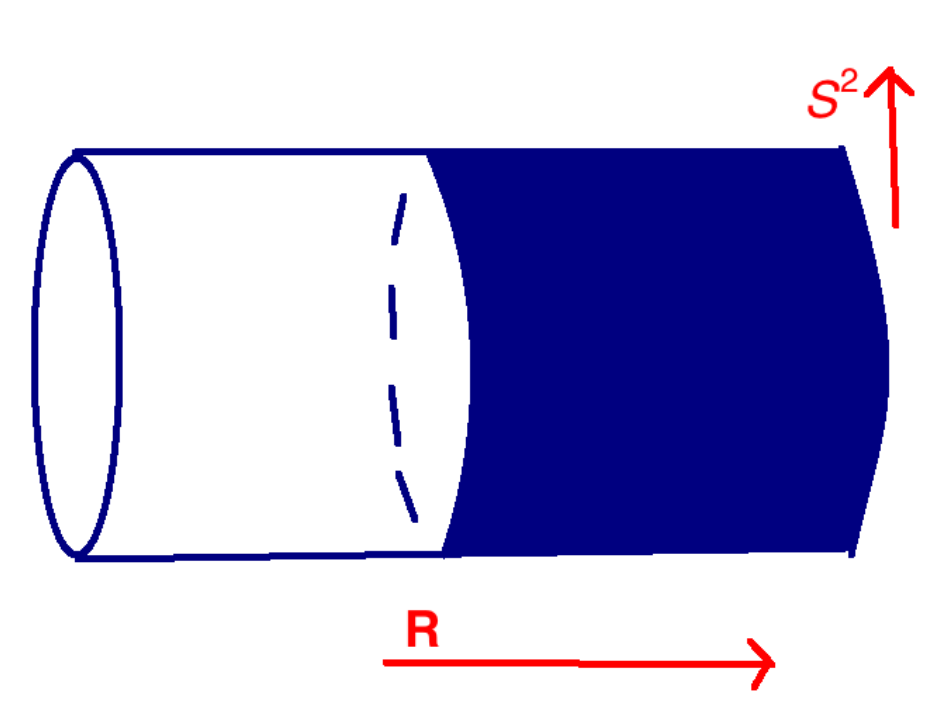
\includegraphics[width=0.50\textwidth]{fig03.png}
  \caption{支承于 $\R\times S^2$ 右半部分的拓扑绝缘体（实色区域）。（原文第 21 页，图 3）}
  \label{support}
\end{figure}

拓扑绝缘体中具有 $\theta=\pi$，在某种意义上应当意味着：当一个 $\U(1)$ 瞬子从拓扑绝缘体外移动到其内部时，路径积分测度变号。
为把这一点讲具体，我们应当设计一个在凝聚态物理中有一定意义、且能以这种方式移动瞬子的思想实验。

我们取空间不是 $\R^3$ 而是 $\R\times S^2$，其中两个维度紧致化为二维球面 $S^2$。（我们完全可以改用 $T^2$ 代替 $S^2$：二维环面对应于两个空间方向上的周期边界条件。）考虑支承在 $\R_+\times S^2\subset \R\times S^2$ 上的拓扑绝缘体（图 \ref{support}），其中 $\R_+\subset \R$ 是半直线 $y\geq 0$。把时间方向也计入——我们用它的一份拷贝 $\R'$（即另一份 $\R$）来参数化——则整个时空为 $\h X= \R'\times \R\times S^2$，而拓扑绝缘体的世界体为 $X=\R'\times \R_+\times S^2$。
% [Tutor Note: 这里选 $S^2$ 而非 $\R^2$ 作空间的两个方向，是为了让磁通量子化：$\int_{S^2}F=2\pi/e$ 给出整数瞬子数；若取非紧的 $\R^2$，磁通无需量子化，$P$ 也不再是整数，思想实验就失去意义。文中的 $\R_+$ 是假想的半无限材料占据区，真实样品当然有限，但边界物理只需考察远离样品另一端的区域。]

考虑一个规范场：它在 $S^2$ 上带一个单位磁通，同时在 $\R'\times \R$ 上带一个单位电通量：
\be\label{zelb} \int_{\R'\times \R}\d t \d x \, F_{01}=\frac{2\pi}{e}. \ee
这样的规范场使
\be\label{elb}\h P=\frac{e^2}{32\pi^2}\int_{\h X}\d^4x\,\epsilon^{\mu\nu\alpha\beta}F_{\mu\nu}F_{\alpha\beta}. \ee
取值为 1。注意这是对整个时空 $\h X=\R'\times \R\times S^2$ 的积分。相比之下，我们把 $P$（式（\ref{zelm}））定义为只对拓扑绝缘体世界体 $\R'\times \R_+\times S^2$ 的类似积分。因此 $\h P$ 是拓扑不变量，而 $P$ 不是。若式（\ref{zelb}）中的单位电通量定域在图 \ref{support} 中很靠左的位置，则 $\h P=1$ 而 $P=0$；若它定域在很靠右的位置，则 $\h P=P=1$。

为在这一语境中考察路径积分测度的公式
\be\label{zont}|Z_\psi|(-1)^\iota \ee
我们应把时间方向紧致化并转到欧几里得号差，因为该公式是在后一情形下导出的。
例如，为计算热配分函数 $\Tr\, \exp(-\beta H)$（其中 $H$ 是系统的哈密顿量），我们应取时间方向为周长为 $\beta$ 的圆周 $S$。
只要电通量深处于拓扑绝缘体内部或外部——总之远离其边界——边界费米子就“看不见”该通量。
一般地（确切地说，对 $\oint_SA$ 的一般取值），边界费米子没有零模，故 $|Z_\psi|>0$。
另一方面，若瞬子在拓扑绝缘体之外——即 $P=0$——则 $\iota=0$；若瞬子在拓扑绝缘体之内——即 $P=1$——则 $\iota=1$。路径积分测度始终为实数，因而保持 $\sT$；但当瞬子被移入拓扑绝缘体时，它从正值光滑地过渡到负值。
$\iota$ 从 0 跳到 1——从而路径积分测度变号——恰好发生在边界狄拉克算子的某个本征值穿过零之时，换言之，发生在 $|Z_\psi|=0$ 之时。
% [Tutor Note: 这段是“$\theta=\pi$”的精确含义：测度随瞬子穿越边界而从 $+$ 变到 $-$，其符号正是 $(-1)^P$。注意 $\iota$ 只能取整数值，故在 $P$ 从 0 连续变到 1 的过程中，必然存在某个中间点使边界狄拉克算子的本征值穿过零、$|Z_\psi|=0$；符号的改变正是通过这个零点完成的，这也说明了为何 $\theta$ 项的相位必须由边界费米子的 $\eta$ 相位来“补”。]

$P=1$ 时路径积分为负，这一事实可以表述为：拓扑绝缘体的路径积分测度包含一个因子 $(-1)^P=\exp(\i\pi P)$。这就为“拓扑绝缘体内部具有 $\theta=\pi$”这一陈述赋予了精确含义。

另一种也许更少技术性的、为“$\theta=\pi$”赋予精确含义的方式已在文献 \cite{RF} 中描述过。让我们回到洛伦兹号差的图像：整个时空为 $\hat X=\R'\times \R\times S^2$，拓扑绝缘体位于 $X=\R'\times \R_+\times S^2$，而边界狄拉克费米子位于 $\partial X\cong \R'\times\{0\}\times S^2$。为求出边界费米子的量子态，我们须求出 $S^2$ 上二维狄拉克算子的本征模，然后将其量子化。在 $S^2$ 上存在单位磁通时，二维狄拉克算子有一个电荷 $-e$、具有某一种二维手征性的零模，以及一个电荷 $+e$、具有相反二维手征性的零模。（这些零模的存在由 Atiyah--Singer 指标定理的二维版本保证。两个零模互为复共轭；复共轭同时反转电荷与二维手征性。）正如 \cite{JR} 中那样，对这些模作量子化会得到一对电荷为 $\pm e/2$ 的态。拓扑绝缘体的边界在被单位磁通穿过时携带半整数电荷，这一事实可以这样理解：设想通过把一个单位电荷的磁单极子拖入拓扑绝缘体来产生这个单位磁通。（我们假定该单极子从图 \ref{support} 中拓扑绝缘体很靠左处出发，其初始态的磁通伸向左侧、不进入拓扑绝缘体。）当单极子进入材料时，其表面出现一个单位磁通，相应地其表面电荷跳变半个整数单位。但当单极子进入拓扑绝缘体时，单极子自身的电荷也会跳变半个整数单位，因为在 $\theta=\pi$ 的世界中磁单极子带有半整数电荷 \cite{Dyons}。在拓扑绝缘体的一个格点模型中确实已经证明：当磁单极子进入拓扑绝缘体时，拓扑绝缘体表面出现半整数电荷，而单极子本身获得半整数电荷 \cite{RF}。这为“拓扑绝缘体具有 $\theta=\pi$”这一说法提供了直接解释。
% [Tutor Note: 半整数电荷的两个来源必须区分：其一是边界上的 $\theta$ 项引起的表面霍尔效应（边界模的分数电荷），其二是体内 $\theta=\pi$ 使磁单极子自身带上半整数电荷（Witten 效应）。原文强调二者同时发生，这是 $\theta=\pi$ 自洽性的直接证据；若只计其一，电荷守恒会被破坏。]

\subsubsection{为什么配分函数等于负一的指标次幂？（Why is The Partition Function Equal to $(-1)^\iota$?）}\label{why}

上述故事的一部分是：在无边紧致四维流形 $X$ 上，带背景 $U(1)$ 规范场 $A$ 时，与拓扑绝缘体相应的拓扑场论的配分函数为 $(-1)^\iota$。读者也许会问，这与拓扑绝缘体的其他已知描述有何关系。

我们采用以下关于拓扑绝缘体与普通绝缘体之间相变的标准刻画：当 $D=4$ 狄拉克费米子 $\psi$ 的质量参数 $m$ 穿过零并变号时，该相变发生。

首先回顾狄拉克算子指标的定义。在定向四维流形上，我们定义手征性算子
\be\label{chiro}\bg=\frac{1}{4!}\eps^{ijkl}\g_i\g_j\g_k\g_l,\ee 其中 $\eps^{ijkl}$ 是 Levi-Civita 张量。我们写 $\psi=\psi_++\psi_-$，其中 $\psi_\pm=\frac{1}{2}(1\pm \bg)\psi$ 满足 $\bg\psi_\pm=\pm\psi_\pm$；并称 $\psi_+$ 与 $\psi_-$ 具有正、负手征性。$\bg$ 与狄拉克算子 $\D$ 反交换，故 $\D$ 把 $\psi_+$ 映到 $\psi_-$，反之亦然。我们用 $n_+$ 表示 $\D$ 作用在 $\psi_+$ 上的零模空间的维数，用 $n_-$ 表示 $\D$ 作用在 $\psi_-$ 上的零模空间的维数。狄拉克算子的指标为 $\iota=n_+-n_-$，这是一个基本的拓扑不变量。
% [Tutor Note: 手征性算子 $\bg$ 的归一化 $1/4!$ 与 $\eps^{ijkl}$ 的约定有关：在四维欧氏空间中 $\eps^{1234}=1$（或 $-1$，取决于约定），$\bg^2=1$、$\{\bg,\g^i\}=0$。若 $\eps$ 的符号取反，$\bg$ 整体变号，$\psi_\pm$ 互换，$n_+-n_-$ 也随之变号——所以“$\iota$ 的符号”本身没有绝对意义，只有 $(-1)^\iota$ 才是与约定无关的物理量。]

为证明 $\iota$ 的拓扑不变性，注意到 $\bg$ 与 $\D$ 反交换：若 $\D\psi=\lambda\psi$ 且 $\lambda\not=0$，则 $\D(\bg\psi)=-\lambda\bg\psi$。因此当 $\lambda\not=0$ 时 $\psi$ 与 $\bg \psi$ 必须线性无关，从而手征投影 $\psi_\pm=\frac{1}{2}(1\pm\bg)\psi$ 均非零。考虑“哈密顿量” $H=\D^2$。$\D$ 的零模与 $H$ 的零模相同；更一般地，满足 $H\psi=E\psi$ 的 $H$ 的本征态是 $\D\psi=\pm\sqrt{E}\psi$ 的解的线性组合。若 $E\not=0$，则 $\D\psi=\pm\sqrt{E}\psi$ 的解具有非零的手征投影 $\psi_\pm$，且二者 $E$ 相同。因此 $H$ 的非零能级成对出现，且一对中正、负手征性各一个。当我们改变 $X$ 上的规范场或度规时，零能态空间可能发生的变化仅仅是：一对相反手征性的态可以移入或移出零能。在此过程中 $n_+$ 与 $n_-$ 改变，但 $\iota=n_+-n_-$ 不变。
% [Tutor Note: 原文此处拼作 “Hamitlonian”，应为 “Hamiltonian”（哈密顿量），译文按正确拼写处理。另外，这一“配对”论证只证明了 $\iota$ 在连续形变下的不变性；要证明它对所有拓扑类不变，还需后文的 Atiyah--Singer 指标公式（\ref{erfo}）。原文有意先给出初等论证，再引入指标定理。]

设 $X$ 与 $A$ 使得 $\iota\not=0$，为确定起见取 $\iota>0$。一般地，当 $\iota>0$ 时 $\psi_+$ 有 $\iota$ 个零模而 $\psi_-$ 没有零模；以下就假定处于这种情形。那么带相反电荷的费米子场 $\bar\psi$ 的零模又如何呢？记 $\bar\psi_-$ 与 $\bar\psi_+$ 为其确定手征性的分量，则 $\bar\psi_-$ 有 $\iota$ 个零模而 $\bar\psi_+$ 没有零模。（$\bar\psi_-$ 的零模是 $\psi_+$ 的零模的复共轭。）

由于这 $2\iota$ 个零模，当 $m=0$ 时费米子路径积分为零。然而当 $m\not=0$ 时，作用量中含有
\be\label{delfo}I=\int\d^4x \left(\dots -m\bar\psi_-\psi_++\dots\right),\ee
相应地，路径积分的被积函数 $e^{-I}$ 含有因子
\be\label{elfo} \exp\left(m\int\d^4x \bar\psi_-\psi_+\right). \ee
展开这一因子，一个 $\bar\psi_-$ 零模与一个 $\psi_+$ 零模可以以贡献一个 $m$ 因子为代价而被“抬升”掉。
% [Tutor Note: 这里的配对是“每个 $\bar\psi_-$ 零模与一个 $\psi_+$ 零模抵消一个 $m$ 因子”：$2\iota$ 个零模给出 $\iota$ 对，故路径积分正比于 $m^\iota$（而不是 $m^{2\iota}$）。因子 $m$ 的幂次直接给出符号的奇偶性——这是 $(-1)^\iota$ 的来源，不需要任何正规化细节。]

于是，对小的 $m$，路径积分正比于 $m^\iota$。因此，若路径积分在比如 $m>0$ 时为正定，则它在 $m<0$ 时的符号为 $(-1)^\iota$。（超出我们所设的零模只会贡献 $m$ 的偶数次幂，故不影响这一符号。）该符号是答案的普适部分，也是人们把拓扑绝缘体作长距离极限后所得拓扑场论的配分函数。
% [Tutor Note: “正比于 $m^\iota$”这一结论只对 $|\iota|$ 个净零模计数；若存在额外的成对零模，它们贡献 $m^2$ 的因子，不改变符号。注意此处 $m$ 是 $D=4$ 狄拉克费米子的质量，与边界 $2+1$ 维费米子的质量无关：前者是体态能隙的参数，后者是边界态的质量项。]

本文后面对若干类似问题会作更精确的处理，其中包括对正规化的说明。例如见第 \ref{bulkboundary} 节。

\subsubsection{指标与配边不变性（The Index And Cobordism Invariance）}\label{cobo}

我们在第 \ref{why} 节定义狄拉克指标 $\iota$ 时，用到了这样的事实：在无边的定向四维自旋流形 $X$ 上，费米子零模的方程 $\D\psi=0$ 分裂为关于手征投影 $\psi_+$ 与 $\psi_-$ 的两个独立方程。

\begin{figure}[htbp]
  \centering
  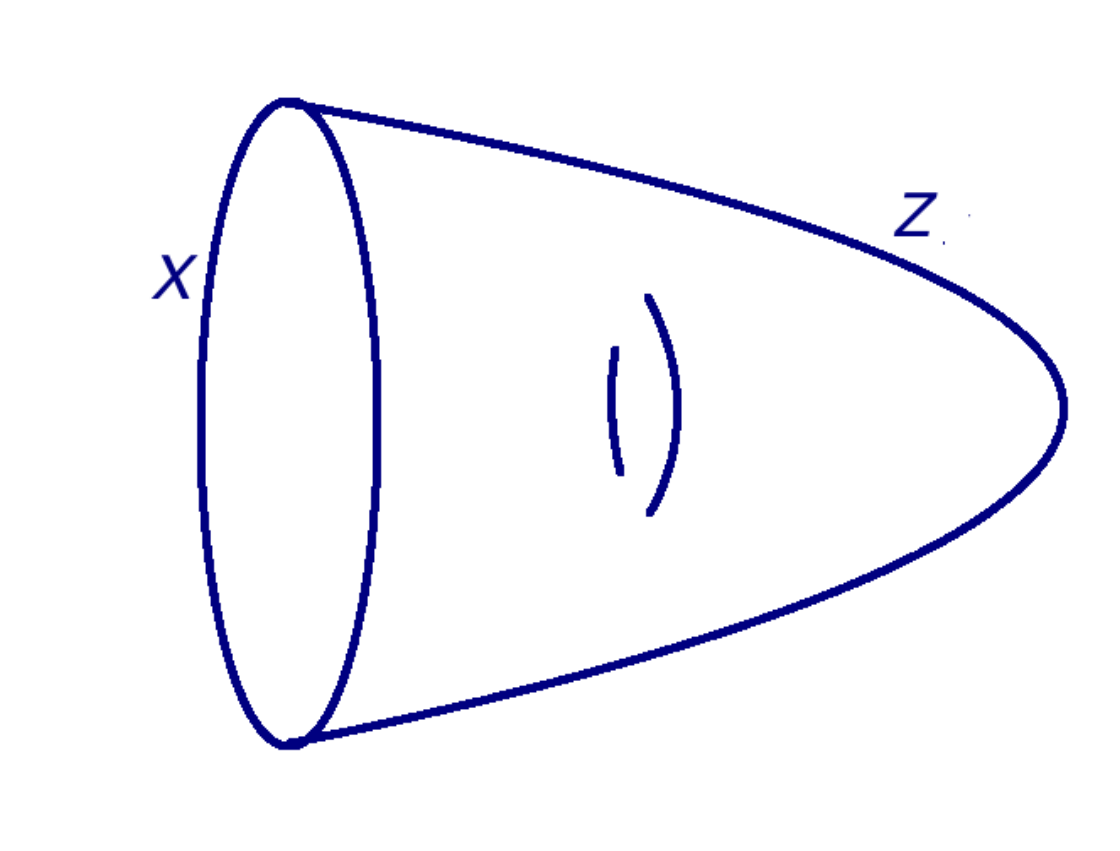
\includegraphics[width=0.55\textwidth]{fig04.png}
  \caption{对流形 $X$ 定义的拓扑不变量 $\iota$，若只要 $X$ 是某个高一维流形 $Z$ 的边界它便为零，则称之为配边不变量。若定义 $\iota$ 时需要 $X$ 具有某种结构（例如定向、自旋结构或 $\U(1)$ 规范场），则要求该结构能延拓到 $Z$ 上。（原文第 25 页，图 4）}
  \label{coob}
\end{figure}

同样的结论对任何偶数维都成立，而原始的 Atiyah--Singer 指标定理 \cite{ASfirst,AS} 给出了 $\iota$ 的上同调公式。
对 $D=4$ 中的 $\U(1)$ 规范场，公式为
\be\label{erfo}\iota=\hA-P.\ee
其中 $P$ 是式（\ref{zelm}）所定义的瞬子数，而
\be\label{ziffy}\hA=-\frac{1}{48}\int_X\,\frac{\tr\,R\wedge R}{(2\pi)^2},\ee
$R$ 是作为矩阵值 2-形式看待的黎曼张量。该公式立即蕴含\footnote{这里我们把原来的逻辑倒过来了。在指标定理的原始证明 \cite{ASfirst} 中，人们先证明指标是配边不变量，再利用这一知识推出它的公式。}：$\iota$ 是配边不变量——若 $X$ 是某个定向五维自旋流形 $Z$ 的边界，且 $\U(1)$ 规范场可延拓到该流形上（图 \ref{coob}），则 $\iota=0$。因为在这种情形下 $\hA=P=0$，故指标为零。例如有
\be\label{wiffy}\hA=-\frac{1}{48}\int_X \,\frac{\tr\,R\wedge R}{(2\pi)^2}=-\frac{1}{48}\int_Z\d \,\frac{\tr\,R\wedge R }{(2\pi)^2}=0\ee
（这里先用斯托克斯定理把 $X$ 上的积分写成 $Z$ 上的积分，再用比安基恒等式 $DR=0$ 证明 $\d\,\tr\, R\wedge R=0$）。类似的论证表明 $P=0$。
% [Tutor Note: 式（\ref{erfo}）把指标拆成“引力部分 $\hA$ 减去瞬子数 $P$”，这里 $\hA$ 是 $\hat A$ 亏格（即 $\hat A$ 示性类在 $X$ 上的积分），而非某个局部密度；$P$ 的归一化使 $S^2\times S^2$ 上单位磁通给出 $1$。符号约定（$\iota=\hA-P$ 而不是 $P-\hA$）与手征性算子的定义及 $n_\pm$ 的指称直接相关，改动其一都会使 $(-1)^\iota$ 不变而 $\iota$ 变号。]

既然 $\iota$ 是配边不变量，$(-1)^\iota$ 也是；我们已经看到，后者正是与拓扑绝缘体相应的体态 sTQFT 在可定向流形上的配分函数。
随着本文的展开将会清楚：与自由费米子物态相应的 sTQFT，其配分函数总是配边不变量。这一点在 \cite{KTTW} 中已有猜想。
一般地，\footnote{简短的说明见 \cite{Freed} 中对式（5.4）的讨论。}从一个这样的 $\U(1)$ 值配边不变量（即从适当的配边群到 $\U(1)$ 的同态）出发，总能构造一个可逆拓扑场论，使该不变量成为其配分函数。这一陈述的粗略想法是：配边不变性蕴含配分函数之间的若干关系，而这些关系正是人们在拓扑场论中会从物理上预期的。此类陈述最简单的例子示于图 \ref{cob}。配边不变性如何蕴含物理性质（幺正性）的另一例子，见第 \ref{rpo} 节末尾。
% [Tutor Note: “从配边不变量构造可逆 TQFT”这一步在数学上对应“可逆 TQFT 由配边群到 $\U(1)$ 的同态分类”这一结果：$D$ 维可逆 TQFT 的等价类可由配边群 $\Omega_D$ 到 $\U(1)$ 的同态刻画。原文说“一般地”，实际依赖的是配边关系的几何实现（每个配边都对应一个可计算的配分函数），而不是任意同态都能实现——这一点在后文讨论 sTQFT 的 spin/pin 结构时会再次出现。]

所有幺正可逆 TQFT 或 sTQFT 是否都与配边不变量相联系，目前似乎尚不清楚。
由于这一点未知，我们其实并不清楚“通常的自由费米子物相与配边不变量相联系”这一事实，究竟只是“它们有能隙、体内没有拓扑序”的推论，还是更为特殊的性质。
无论如何，配边不变性比拓扑不变性强得多。
% [Tutor Note: 这句“配边不变性比拓扑不变性强得多”是本节的方法论要点：拓扑不变性只要求不变量在微分同胚下不变；配边不变性还要求它在流形作为高一维流形的边界时取平凡值，从而给出切割--黏合关系。后者正是构造可逆 TQFT 所需的全部数据。]

\begin{figure}[htbp]
  \centering
  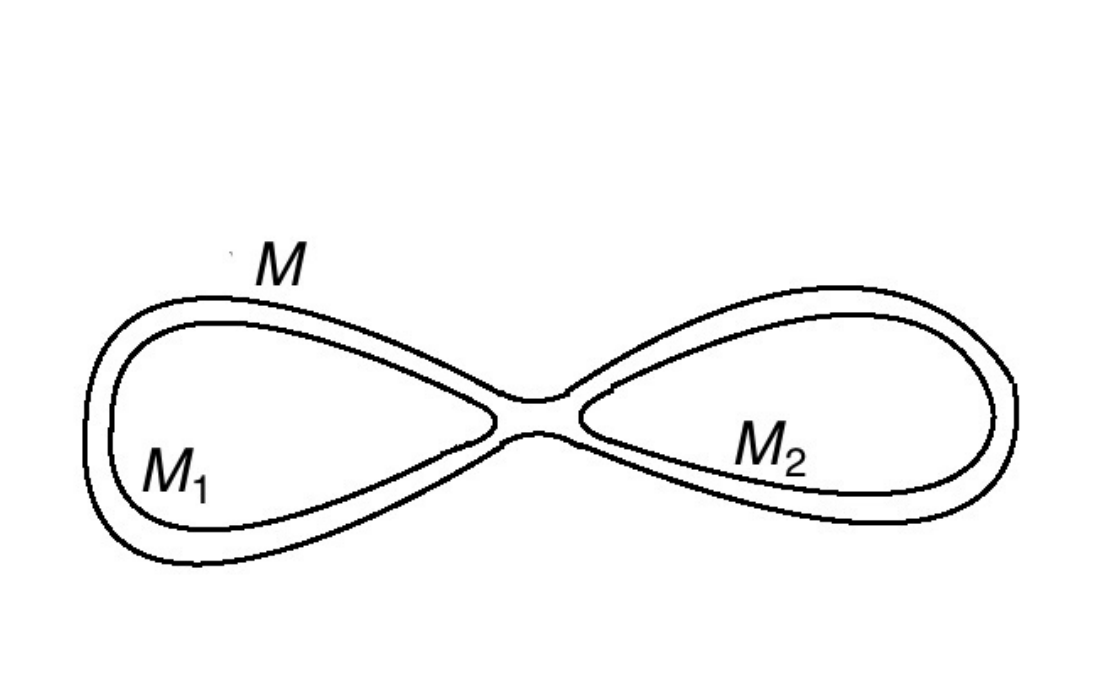
\includegraphics[width=0.60\textwidth]{fig05.png}
  \caption{这里给出“配边不变性导致拓扑场论中自然的关系”这一陈述的最简单图示。两个 $D$ 维流形 $M_1$ 与 $M_2$ 的\emph{连通和} $M$ 是这样作出的：从 $M_1$ 与 $M_2$ 中各挖去一个小洞，再沿各自的边界把它们黏合起来。若球面 $S^{D-1}$ 上物理态的空间是 1 维的（幺正拓扑场论中理应如此），则可推出配分函数之间的一个普适关系：$Z_M = g Z_{M_1}Z_{M_2}$，其中 $g$ 是该理论的特征常数。配边不变性给出 $g=1$ 的这种关系，因为 $M$ 与 $M_1$ 和 $M_2$ 的无交并配边。该配边示意于本图（取 $D=1$、所有流形均为圆周的情形）。由配边不变量得到的拓扑场论总满足如下条件：任意 $D-1$ 维流形上物理态空间的维数为 1；这正是它们给出上述类型关系的原因。（原文第 27 页，图 5）}
  \label{cob}
\end{figure}
